\chapter{Искусство}

\section{Художники}
\subsection{Виктор Михайлович Васнецов}
% https://muzei-mira.com/biografia_hudojnikov/765-viktor-mihaylovich-vasnecov-biografiya.html
В\'{и}ктор Мих\'{а}йлович Васнец\'{о}в родился в 1848 году 15 мая в селе со смешным названием Лопьял. Отец Васнецова был священником, также как и его дед и прадед. В 1850 году Михаил Васильевич увёз семью в село Рябово. Это было связано с его службой. У Виктора Васнецова было 5 братьев, один из которых также стал знаменитым художников, звали его Аполлинарий.

Талант Васнецова проявился с детства, но крайне неудачное \explainDetail{денежное}{д\'{е}нежный/-ая/-ое}{monetary} положение в семье не оставило вариантов, как отдать Виктора в Вятское духовное училище в 1858 году. Уже в 14-летнем возрасте Виктор Васнецов учился в Вятской духовной семинарии. Детей священников туда брали бесплатно.

Так и не окончив семинарию, в 1867 году Васнецов отправился в Петербург поступать в Академию художеств. Денег у него было совсем мало, и Виктор выставил на «аукцион» 2 свои картины -- «Молочница» и «Жница». До \explainDetail{отъезда}{отъезд}{departure} он так и не получил за них денег. 60 рублей за эти две картины он получил спустя несколько месяцев уже в Петербурге. \explainDetail{Прибыв}{прибывать/прибыть}{arrive} в столицу, у молодого художника было всего 10 рублей.

Васнецов отлично справился с экзаменом по рисованию и сразу \explain{был зачислен}{was enrolled (зачисл\'{я}ть/зач\'{и}слить: to enrol, to enlist)} в Академию. Около года он занимался в Рисовальной школе, где и познакомился со своим учителем -- И. Крамским.

К занятиям в Академии художеств Васнецов приступил в 1868 году. В это время он \explain{сдружился с}{made friends with} Репиным, и даже одно время они жили на одной квартире.

Хоть Васнецову и нравилось в Академии, но он её не закончил, уехав в Париж в 1876 году, где прожил больше года. В это время там же находился и Репин в \explainDetail{командировке}{командировка}{business trip}. Они также поддерживали дружеские отношения.

После возвращения в Москву Васнецова сразу приняли в Товарищество передвижных художественных выставок. К этому времени стиль рисования художника значительно меняется, да и не только стиль, сам Васнецов перебирается жить в Москву, где сближается с Третьяковым и Мамонтовым. Именно в Москве Васнецов \explainDetail{раскрылся}{раскрыв\'{а}ться/раскр\'{ы}ться}{to open, uncover oneself, to come out}. Ему нравилось находиться в этом городе, он чувствовал себя легко и \explainDetail{выполнял}{выполн\'{я}ть/в\'{ы}полнить}{to perform, execute, carry out} различные творческие работы.

Более 10 лет Васнецов \explainDetail{оформлял}{оформл\'{я}ть/оф\'{о}рмить}{put into shape, form} Владимирский соб\'{о}р в Киеве. В этом ему помогал М. Нестеров. Именно после окончания этой работы, Васнецова можно по праву назвать великим русским иконописцем.

1899 год стал \explainDetail{пиком}{пик}{peak} популярности художника. На своей выставке Васнецов представил публике «Трёх богатырей».

После революции Васнецов стал жить уже не в России, а в СССР, что его серьёзно \explainDetail{угнетало}{угнетать}{opress, depress, despirit}. Люди \explainDetail{уничтожали}{уничтож\'{а}ть/уничт\'{о}жить}{to destroy, obliterate; уничтож\'{е}ние: destruction} его картины, \explainDetail{относились}{относ\'{и}ться + \textit{дат.}}{to treat} неуважительно к художнику. Но до конца своей жизни Виктор Михайлович был в\'{е}рен своему делу -- он рисовал. \explainDetail{\'{У}мер}{умирать/умереть}{умир\'{а}ю, умир\'{а}ешь, умир\'{а}ют; умр\'{у}, умрёшь, умр\'{у}т: to die} он 23 июля 1926 года в Москве, так и не закончив портрет своего друга и ученик\'{а} М. Нестерова.



\subsection{Лики России Виктора Васнецова}

17 января в Центральной районной библиотеке им. А. П. Чехова прошла интерактивная лекция «\explainDetail{Лики}{лик}{character (like in a book)} России Виктора Васнецова»

Виктор Васнецов был известным мастером бытовой и исторической живописи. Его картины \explain{приобретали}{acquired} коллекционеры Павел Третьяков и Савва Мамонтов. Полотн\'{о} Васнецова «Богатыри» стало одним из первых обращений к был\'{и}нному сюжету в истории русской ж\'{и}вописи. Кроме нап\'{и}сания картин, Васнецов делал иллюстрации к книгам, создавал эскизы архитект\'{у}рных \explainDetail{сооружений}{сооружение}{construction, building, erection} и расписывал хр\'{а}мы в разных городах России.

Родился Виктор Васнецов 15 мая 1848 года в Вятской губернии (сегодня --- Кировская область) в семье священника. Родители старались дать детям \explainDetail{разностороннее}{разносторонний}{many-sided, versatile} образование: читали им научные журналы, учили рисованию. Первыми работами Виктора Васнецова были пейзажи, сюжеты сельской жизни. Природа на его картинах во многом списана с вятских видов: \explain{изв\'{и}листые}{meandering} реки, холм\'{ы}, \explainDetail{густые}{густой}{thick, dense} \explainDetail{хвойные}{хвойный}{coniferous (adj.); хв\'{о}я: coniferous} леса.

В 1858 году Васнецов поступ\'{и}л в дух\'{о}вное училище, затем -- в семинарию. Он изучал \explainDetail{жити\'{я}}{жити\'{е}}{life of a saint} свят\'{ы}х, хронографы, летописные своды, \explainDetail{пр\'{и}тчи}{пр\'{и}тча}{parable}. Древнерусская литература зародила в художнике интерес к старин\'{е}.

В свободное от учёбы время Васнецов рисовал портреты горож\'{а}н, делал по памяти зарис\'{о}вки, помогал расписывать Вятский кафедральный собор. В 1867 году он проиллюстрировал книгу этнографа Николая Трапицина о пословицах. Позже художник опубликов\'{а}л свои рисунки \explain{отдельно}{separately} -- в альбоме «Русские \explainDetail{пословицы}{посл\'{о}вица}{proverb, saying, adage} и \explainDetail{поговорки}{поговорка}{посл\'{о}вица} в рисунках В.М. Васнецова». В годы учёбы живописец создал первые пол\'{о}тна «Жница» и «Молочница».

В 1867 году Виктор Васнецов бр\'{о}сил семинарию и уехал в Петербург. Зимой этого года он занимался живописью в школе своего друга -- художника Ивана Крамского, а спустя год, поступил в Петербургскую академию художеств.

В академии Васнецов получил две малые серебряные медали за уч\'{е}бные работы, а через два года ему \explainDetail{вручили}{вруч\'{а}ть/вруч\'{и}ть}{to hand over, to deliver, to present,  to entrust} Большую серебряную медаль за картину «Христос и Пилат перед народом». В это время художник рисовал иллюстрации к сказкам и литературно-педагогическим трудам Николая Столпянского -- «Народная азбука», «Солдатская азбука». Во время жизни в Петербурге Виктор Васнецов создавал пол\'{о}тна бытового жанра -- «\explainDetail{Н\'{и}щие}{н\'{и}щий}{beggar} певцы», «С квартиры на квартиру», «Рабочие с т\'{а}чками». В 1874 году живописец получил бронзовую медаль на Всемирной выставке в Лондоне за картины «Книжная лавка» и «Мальчик с бутылкой вина».

После окончания академии художник уехал с друзьями за гран\'{и}цу. Там прод\'{о}лжил писать, участвовал в выставках и салонах. В парижской \explainDetail{мастерск\'{о}й}{мастерск\'{а}я}{workshop} своего др\'{у}га Василия Поленова Васнецов \explainDetail{наброс\'{а}л}{набр\'{а}сывать/наброс\'{а}ть}{to sketch, to draw an outline (набр\'{о}сок: sketch)} эскиз картины «Богатыри» -- первого полотн\'{а} по мотивам русских былин.

Васнецов прожил за границей около года, в 1877 году вернулся в Москву. Здесь познакомился с коллекционером Павлом Третьяковым, часто бывал на музыкальных вечерах в его семье.

В московский период художник писал картины с сюжетами из истории и сказок Древней Руси. Одно из первых пол\'{о}тен - «После \explainDetail{побоища}{побоище}{carnage} Игоря Святославича с половцами» -  экспонировалось на VIII выставке \explainDetail{передвижников}{передв\'{и}жник}{wanderer}. Картину купил Павел Третьяков.

Познакомился Васнецов и с меценатом Саввой Мамонтовым, стал участником его Абрамцевского кр\'{у}жка. Мамонтов \explainDetail{предлож\'{и}л}{предлаг\'{а}ть/предлож\'{и}ть}{to offer, to propose, to suggest} художнику напис\'{а}ть три картины для интерьера управления Донецкой железной дороги. Так появились пол\'{о}тна «Битва скифов со славянами\footnote{Battle of the Scythians with the Slavs}», «Ковёр-самолёт», «Три царевны подземного царства». Однако чл\'{е}ны \explainDetail{правления}{правление}{reign} отказались от пол\'{о}тен со сказочными сюжетами. Картины выкупили Савва Мамонтов и его брат.

Виктор Васнецов много бывал в Абрамцеве в ус\'{а}дьбе мецената, писал портреты членов его семьи. \explainDetail{Окр\'{е}стности}{окр\'{е}стности}{surroundings} Абрамцева появились и на других картинах Васнецова: березовые \explainDetail{р\'{о}щи}{р\'{о}ща}{grove} и изв\'{и}листые р\'{е}чки, \explainDetail{овр\'{а}ги}{овр\'{а}г}{deep narrow valley} и пруды, поросшие осокой. Здесь в 1880 году художник напис\'{а}л «Алёнушку».

Виктор Васнецов пр\'{о}бовал себя и в архитектуре. Он с\'{о}здал эскизы для \explainDetail{постр\'{о}ек}{постр\'{о}ека}{construction} в усадьбе Мамонтовых, по рисункам Васнецова и Поленова в Абрамцеве построили церковь Сп\'{а}са Нерукотв\'{о}рного. Также художник нарисов\'{а}л эскизы собственного дома-мастерской, \explainDetail{особняк\'{а}}{особн\'{я}к}{mansion} Ивана Цветкова, главного фасада Третьяковской галереи в Лаврушинском переулке в Москве.

В начале 1885 года профессор Петербургского университета Адриан Прахов, один из учител\'{е}й Васнецова, предлож\'{и}л ему расписать \explain{только что построенный}{just/newly built} Владимирский собор в Киеве. Васнецов называл \explain{р\'{о}спись}{(\textit{ж.р.}) painting, mural} хр\'{а}ма главной работой своей жизни -- он \explainDetail{посвят\'{и}л}{посвящ\'{а}ть/посвят\'{и}ть}{devote, dedicate [посвящ\'{а}ю, -\'{а}ешь, -\'{а}ют; посвящ\'{у}, посвят\'{и}шь, посвят\'{я}т]} ей около 11 лет. Художник говорил: «Нет на Руси для русского художника \explain{свят\'{е}е}{holier $<$ свят\'{о}й: holy, sacred} и \explain{плодотворнее}{more fruitful (плодотв\'{о}рный)} дела, как украшение хр\'{а}ма». Во время работы Виктор Васнецов изучал памятники раннего христианства в Италии, фрески Софийского соб\'{о}ра в Киеве, использовал знания иконописи и храмового \explainDetail{зодчества}{з\'{о}дчество}{ (dated) architecture}, пол\'{у}ченные в семинарии.

Всего было с\'{о}здано около 400 эскизов, расписано св\'{ы}ше 2000 квадратных метров. Собор освятили в 1896 году \explain{в присутствии}{in the presence of} императора Николая I и его семьи. После Владимирского собора художник расписывал храмы в Петербурге, \explainDetail{Гусь-Хрустальном}{Гусь-Хрустальный}{town in Vladimir Oblast}, Дармштадте, Варшаве.

До конца жизни Виктор Васнецов продолжал пис\'{а}ть картины по мотивам сказок. В 1898 году он закончил полотн\'{о} «Богатыри», над которым работал 25 лет.

Виктор Васнецов \explainDetail{\'{у}мер}{умир\'{а}ть/умер\'{е}ть}{to die; past tense: умер\'{а}л/\'{у}мер} в своей мастерск\'{о}й в 1926 году. Художника похорон\'{и}ли на Введенском \explain{кл\'{а}дбище}{cemetery} в Лефортово.


\subsection{Василий Васильевич Кандинский}
% https://muzei-mira.com/biografia_hudojnikov/2022-vasiliy-vasilevich-kandinskiy.html
Знаменитый создатель легендарного «Синего \explainDetail{всадника}{всадник}{rider}» обратился к сфере искусств \explain{относительно}{relatively} поздно -- в возрасте около 30 лет, что не помешало ему достичь значительных высот, став одним из создателей абстракционизма, основателем многочисленных художественных \explainDetail{объединений}{объединение}{union} и педагогом в Высшей школе строительства и художественного конструирования, более известной как Баухаус.

Кандинский происход\'{и}л из оригинального купеческого сибирского рода, где \explain{прич\'{у}дливо}{bizarrely} смешалась кровь тунгусских князей с древнейшей \explain{родословной}{pedigree}, не менее старинного княжеского рода манси и каторжников, \explainDetail{с\'{о}сланных}{с\'{о}сланный}{exiled ($<$ ссыслать/сослать)} в Нерчинск за \explain{Бог весть}{God knows} какие \explainDetail{провинности}{провинность (женский род)}{delinquency, fault}.

В детстве будущего художника его семейство много путешествовало по Европе и территории России, а затем \explain{поселилось}{settled} в Одессе, которая тогда была третьим по \explain{значимости}{significance} городом Российской империи. В этом чудесном южном городе Василий закончил гимназию, а также получил музыкальное и художественное образование. Несмотря на \explain{несомненное}{undoubted} \explain{даров\'{а}ние}{gifting, endowment, ability} мальчика, родители \explain{пр\'{о}чили}{intend, predict} ему карьеру юриста, что он и воплотил в жизнь, \explain{учась}{learning} с \explainDetail{перерывами}{перерыв}{break} в Московском университете.

Однако настоящая жизнь Кандинского как художника начинается с выставки импрессионистского искусства в Москве 1895 года, где его в самое сердце \explainDetail{поразила}{поражать/поразить}{to amaze, affect, stagger, startle} работа Клода Моне.
В следующем году он уезжает в Мюнхен, где \explain{погружается}{sinks, dives, plunges} в среду экспрессионизма, но н\'{а}чало Первой Мировой войны прерывает его становление и он возвращается на родину. Но с Советской Россией ему не по пути, и Василий Васильевич в 1921 году навсегда покидает родные пенаты. Он уезжает в Германию, откуда через некоторое время вместе с женой бежит во Францию от нацистов, закрывших Баухаус и признающих только \explain{собственное}{own}, глубоко формализованное и статичное искусство. В принявшей его стране он получает гражданство, становится известным и живет всю свою оставшуюся жизнь.

За годы своего творчества Кандинский основал объедин\'{е}ние «Фал\'{а}нга», школу, \explainDetail{участвовал}{участвовать/поуч\'{а}ствовать}{participate} в «\explainDetail{Бубновом валете}{Бубновый валет}{Jack of diamonds}», затем \explainDetail{заложил}{закл\'{а}дывать/залож\'{и}ть}{to put, to lay, to place ( залож\'{и}ть стран\'{и}цу: to mark a page, to put in a bookmark); to lay the foundations of; } Новое мюнхенское художественное объединение, а позже -- и знаменитый «Синий всадник».

В начале своей художественной карьеры мастер работал в реалистичной и \explain{частично}{partialy} абстрактной манере, экспериментировал с формами и цветом, писал на стекле.

Начав преподавательскую деятельность, Кандинский \explain{вск\'{о}ре}{soon} стал видным теоретиком абстракционизма и Баухауса. Его самые известные \explainDetail{пол\'{о}тна}{полотн\'{о}}{linen, canvas} -- это «Москва», «Восток», «Колебание» и «Композиция», одн\'{а}ко их очень много и каждое из них имеет п\'{о}лное право называться настоящим шедевром. Его картины \explain{исключительно}{exceptionally, exclusively} интересно рассматривать, \explainDetail{возникает}{возник\'{а}ть/возн\'{и}кнуть}{to arise, to appear, to emerge, to originate, to spring up} \explain{ощущение}{sensation, feeling}, что с каждой точки зрения в них открывается что-то новое и необычное.

К сожалению, пришедшие к власти фашисты успели уничтожить множество работ Василия Васильевича, как и других талантливых мастеров, причисленных к категории «дегенеративного искусства». Но и оставшихся пол\'{о}тен нам достаточно, чтобы понимать, каким великим талантом был Кандинский. \explainDetail{Скончался}{скончаться}{to pass away} мастер в 1944 году в Нейи, \explainDetail{пр\'{и}городе}{пр\'{и}город}{suburb} Парижа.


\section{Произведения}
\subsection{Картина «Три Богатыря» ВМ Васнец\'{о}ва}
% https://muzei-mira.com/kartini_russkih_hudojnikov/1321-opisanie-kartiny-bogatyri-tri-bogatyrya-vasnecova-1898.html

Картина В\'{и}ктора Мих\'{а}йловича Васнец\'{о}ва «Богатыр\'{и}» \explain{по пр\'{а}ву}{rightfully } считается настоящим народным \explainDetail{шед\'{е}вром}{шед\'{е}вр}{masterpiece} и с\'{и}мволом отечественного искусства. \explainDetail{Создав\'{а}лась}{создаваться/создаться}{create} картина во второй половине XIX века, когда среди русских художников был\'{а} очень популярна тема народной культуры, русского фольклора. Для многих художников это увлечение оказалось кратковременным, но у Васнецова народная фольклорная тематика \explainDetail{ст\'{а}ла}{стать/становиться}{become (ст\'{а}л/-а/-о)} \explainDetail{осн\'{о}вой}{осн\'{о}ва}{basis} всего \explainDetail{творчества}{творчество}{cretativity}.

На картине «\explainDetail{Богатыр\'{и}}{богат\'{ы}рь}{A bogatyr or витязь is a stereotypical fictional character in medieval Russian legends}» \explainDetail{изображен\'{ы}}{изображён/-\'{а}/-\'{о}}{depicted; изображение: image, depiction; изображ\'{а}ть/изобраз\'{и}ть: to depict} три русских богатыр\'{я}: Илья Муромец, Добрыня Никитич и Алёша Попович -- знаменитые герои народных \explainDetail{был\'{и}н}{был\'{и}на}{epic}.

\explainDetail{Испол\'{и}нские}{испол\'{и}нский}{gigantic} фигуры богатыр\'{е}й и их коней, распол\'{о}женные \explain{на пер\'{е}днем пл\'{а}не}{in the foreground (пер\'{е}дний пл\'{а}н)} картины, символизируют силу и мощь русского народа. Этому \explainDetail{впечатлению}{впечатл\'{е}ние}{impression} \explainDetail{спос\'{о}бствуют}{способствовать/поспособствовать}{contribute to} и \explainDetail{внушительные}{внушительный}{impressive} размеры картины -- 295$\times$446 см.

Над созданием этой картины художник работал почти 30 лет. В 1871 году был с\'{о}здан первый \explain{набр\'{о}сок}{sketch} сюжета в карандаш\'{е}, и с тех пор художник увлёкся идеей создания этой картины. В 1876 году был сделан знаменитый \explain{эск\'{и}з}{sketch} с уже \explainDetail{н\'{а}йденной}{н\'{а}йденный/-ая/-ое}{$<$ найти} основой композиционного решения. Работа над самой картиной длилась с 1881 по 1898 год. Готовая картина была куплена П. Третьяковым, и до сих пор она \explainDetail{украш\'{а}ет}{украш\'{а}ть/укр\'{а}сить}{decorate} Государственную Третьяковскую галерею в Москве.

\begin{wrapfigure}{l}{0.5\textwidth}
    \begin{center}
        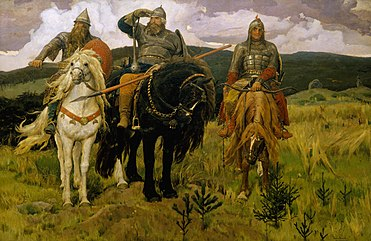
\includegraphics[width=0.49\textwidth]{img/tri_bogatyrya.jpg}
    \end{center}
    \caption{Картина «Три Богатыря» ВМ Васнец\'{о}ва (слева направо: Добрыня Никитич, Илья Муромец и Алёша Попович), ВикипедиЯ.}
\end{wrapfigure}
В центре картины изображён Илья Муромец, народный любимец, герой русских был\'{и}н. Не всем известно, что Илья Муромец не сказочный персонаж, а реальное историческое лицо. История его жизни и \explainDetail{р\'{а}тных}{р\'{а}тный}{military} \explainDetail{п\'{о}двигов}{п\'{о}двиг}{exploit, feat} -- это реальные события. \explain{Впосл\'{е}дствии}{subsequently}, закончив свои труды по охране родины, он стал монахом Киево-Печёрского монастыр\'{я}. Был причислен к л\'{и}ку свят\'{ы}х\footnote{was canonised}. Васнецов эти факты знал, создав\'{а}я образ Ильи Муромца. «\explainDetail{Матёр}{матёрый}{mature, fully grown, hardened} человек Илья Муромец» -- говорит былина. А на картине Васнецова мы видим могучего воина и при том \explainDetail{бесх\'{и}тростного}{бесх\'{и}тростный}{ingenuous, silly} открытого человека. В нём \explainDetail{сочетаются}{сочетаться}{combine} исполинская сила и \explain{великод\'{у}шие}{generosity, magnanimity, goodness}. «А конь под Ильёй \explain{лютый}{fierce} зверь» -- продолжает сказание. \explainDetail{Мощная}{мощный/-ая/-ое}{powerful} фигура коня, изображённого на картине с массивной металлической цепью вместо упряжки, \explainDetail{свид\'{е}тельствует}{свид\'{е}тельствовать}{testify; свидетель: witness} об этом.

Добрыня Никитич по народным преданиям был очень образ\'{о}ванным и \explainDetail{м\'{у}жественным}{м\'{у}жественный}{manly} человеком. С его личностью связано много чудес, наприм\'{е}р, заговорённая броня\footnote{charmed armor} на его плечах, \explain{волш\'{е}бный}{magic} меч-кладенец. Добрыня изображён таким как и в былинах -- величавым, с тонкими, благородными чертами лица, подчёркивающими его культурность, образ\'{о}ванность, \explain{решительно}{decisively} вынимающий меч из \explain{н\'{о}жен}{sheath} с готовностью \explainDetail{бр\'{о}ситься}{брос\'{а}ться/бр\'{о}ситься}{rush} в бой, защищая свою родину.

Алёша Попович \explain{по сравнению с}{as compared with} товарищами молод и строен. Он изображён с \explainDetail{л\'{у}ком}{лук}{bow} и стрелами в руках, но \explain{прикреплённые}{attached} к \explainDetail{седлу}{седло}{saddle} гусли свидетельствуют о том, что он не только бесстрашный воин, но и \explain{гусляр}{player of the musical instrument ``gusli''}, песенник, весельчак. В картине много таких деталей, которые характеризуют образы её персонажей.

Упряжки коней, одежда, амуниция не \explainDetail{вымышленные}{в\'{ы}мышленный/-ая/-ое}{imaginary, fictitious}. Такие образц\'{ы} художник видел в музеях и читал их описания в исторической литературе. Художник \explain{мастерски}{masterfully} передаёт состояние природы, как бы предвещающей о наступлении опасности. Но богатыри представляют собой \explainDetail{надёжную}{надёжный/-ая/-ое}{reliable} и мощную силу защитников родной земли.




\subsection{Картина «Алёнушка» ВМ Васнец\'{о}ва}
% https://muzei-mira.com/kartini_russkih_hudojnikov/1321-opisanie-kartiny-bogatyri-tri-bogatyrya-vasnecova-1898.html

Алёнушка, печальная девочка у \explainDetail{пруда}{пруд}{pond} --- одна из любимых всеми картин В. Васнецова. Художник уд\'{а}чно использует сказочный сюжет, чтобы \explainDetail{раскрыть}{раскрывать/раскрыть}{to open/to discover} сложный и неоднозначный русский характер.

\begin{wrapfigure}{l}{0.4\textwidth}
    \begin{center}
        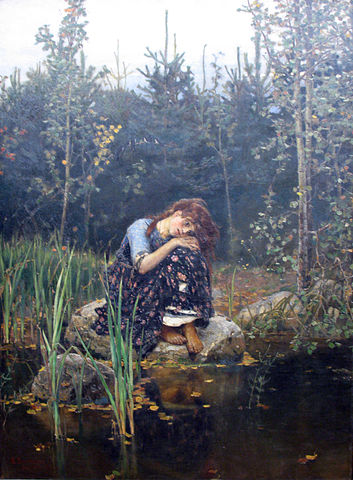
\includegraphics[width=0.38\textwidth]{img/alyonushka.jpg}
    \end{center}
    \caption{Алёнушка, ВикипедиЯ}
\end{wrapfigure}
Грусть девочки очень взрослая. Печаль в её глазах граничит с \explainDetail{отчаянием}{отч\'{а}яние}{despair}. Неубранные рыжие волосы, тёмные глаза, нежно-алые губы --- формируют легко читаемый образ ребёнка с тр\'{у}дной судьб\'{о}й.
В Алёнушке совсем нет ничего \explainDetail{сказочного}{сказочный}{fabulous, fairytale-like}, фантастического.
С\'{о}бственно, вся ск\'{а}зочность сюжета подчеркнута лишь одной деталью --- группой \explainDetail{ласточек}{л\'{а}сточка}{swallow}, сидящих над головой \explainDetail{героини}{героиня}{heroine}. Этим с\'{и}мволом (как известно, л\'{а}сточки символиз\'{и}руют над\'{е}жду) художник \explainDetail{уравновешивает}{уравновешивать/уравновесить}{to balance --- уравнов\'{е}шиваю/-ешь/-ют; уравнов\'{е}шу/-ишь/-ят} полный \explainDetail{тоск\'{и}}{тоск\'{а}}{yearning, longing} \'{о}браз героини, даёт надежду на счастливый финал старой русской сказки.

Васнецов нап\'{о}лнил \explain{ф\'{о}новый}{background} пейзаж атмосферой тишины и гр\'{у}сти.
Отлично удал\'{и}сь художнику в\'{о}дная \explain{гладь}{smooth surface} пруда, \explainDetail{камыш\'{и}}{камыш}{reed}, осока, \explainDetail{ели}{ель}{fir tree}.
Всё \explainDetail{неподв\'{и}жно}{неподв\'{и}жный/-ая/-ое}{still, motionless}, тихо, спокойно.
Даже пруд отраж\'{а}ет героиню очень деликатно, \explain{слегк\'{а}}{slightly}.
Чуть трепещут молодые \explainDetail{ос\'{и}ны}{ос\'{и}на}{aspen}. \explainDetail{Едва}{едв\'{а}}{barely, hardly} \explain{хмурится}{turns gloomly} ос\'{е}ннее небо.
Тёмные, зелёные тона пейзажа контрастируют с \explainDetail{румянцем}{румянец}{blush} на лице героини, а ос\'{е}нняя грусть --- с яркими цветами на юбке Алёнушки. Зритель чувствует: ещё мгнов\'{е}ние и сказка прод\'{о}лжится\dots







\subsection{Картина «Витязь на распутье»}

Виктор Михайлович Васнецов с циклом работ, \explain{посвященных}{dedicated (посвященный + \textit{дат.})} сюжетам русских сказок и былин, оказался \explainDetail{новатором}{новатор}{innovator} в этой области \explainDetail{изобразительного искусства}{изобраз\'{и}тельное искусство}{visual art}. За ним закрепилась репутация «художника-сказочника», он настолько проникся духом русской старины и былинного времени, что свой московский дом построил в виде деревянной избы (сейчас там находится мемориальный музей \explainDetail{живоп\'{и}сца}{живоп\'{и}сец}{painter, artist}).


Картина «В\'{и}тязь на расп\'{у}тье» \explain{отч\'{а}сти}{partly} является и отражением судьбы Васнецова.
Будучи \explainDetail{пр\'{и}знанным}{пр\'{и}знанный}{recognised} художником-передвижником, он, как и его товарищи, \explainDetail{исполнял}{исполнять/исполнить}{performed} жанровые композиции в духе остросоциальных тем, волновавших общество в 1870-1890-х.
Но завладевшая им сказочная тематика диктовала \explainDetail{ин\'{о}е}{ин\'{о}й/ин\'{а}я/ин\'{о}е}{(определительное местоимение) другой, отличный от данного; (неопределённое местоимение) некоторый. See \href{https://ru.wiktionary.org/wiki/\%D0\%B8\%D0\%BD\%D0\%BE\%D0\%B9}{wikictionary.org:иной}.} развитие творчества. Живописец уход\'{и}л от проблем современности и \explain{погружался}{plunge, dive} в мир русской старины, рискуя быть \explainDetail{осужденным}{осужденный}{convicted}.

\begin{wrapfigure}{l}{0.58\textwidth}
    \begin{center}
        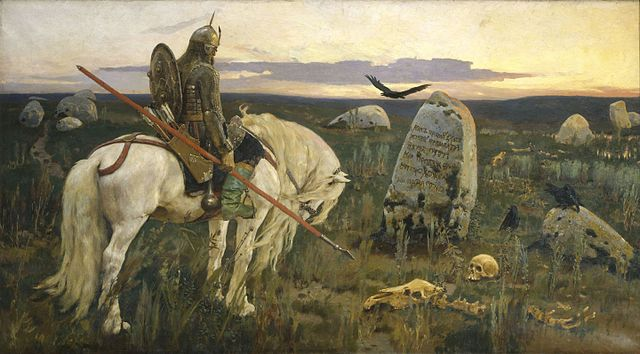
\includegraphics[width=0.57\textwidth]{img/TheKnightAtTheCrossroads.jpg}
    \end{center}
    \caption{Витязь на распутье, ВикипедиЯ}
\end{wrapfigure}
Выбор пути как один из \explain{роков\'{ы}х}{fatal} вопросов человеческой жизни на крупноформатном \explainDetail{холсте}{холст}{canvas} мастера приобрел эпическое звучание.
Перед камнем-предсказателем согнулся под тяжестью фатального \explainDetail{пророчества}{пророчество}{prophecy} опечаленный витязь. \explainDetail{Зловещий}{зловещий}{sinister} в\'{о}рон, садящееся красное солнце нагнетают\footnote{build up the atmosphere} атмосферу. \explainDetail{Нам\'{е}ренный}{нам\'{е}ренный}{intentional} отказ от \explainDetail{изображения}{изображение}{depiction} дороги (как выхода из трудности) художником сделан для того, чтобы показать \explain{неотврат\'{и}мость}{inevitability} судьбы.